\subsection{Petri Nets}

\subsubsection{Logical And}

\descriptionproblem
Define a Petri Net (P/T net) model for calculating the logical conjunction of two variables, $x$, and $y$, each of which takes the values \emph{true} or \emph{false}, with each variable's value being independent of the other.

\questionproblem
\begin{enumerate}
    \item Draw the diagram describing the aforementioned P/T ned model.

    \item Define a P/T net that computes the negation of $x$, which again takes only the values \emph{true} and \emph{false}.
    
    \item Define a P/T net that computes $!\left(x \land y\right)$ by composing the previous models.
\end{enumerate}

\solution
\textbf{\underline{Solution 1}.} We use a Petri Net to describe distributed systems. In other words, it is a soft UML graph with an exact mathematical definition of its execution semantics.


The exercise requests that we design a P/T net that describes the logic and operator (conjunction of two variables): $x \land y$. The values of the variables are their domain, \emph{true} and \emph{false}, and then they are boolean values. The values to try depend on the logic table:

\begin{table}[!htp]
    \centering
    \begin{tabular}{@{} c c c @{}}
        \toprule
        $x$ & $y$ & $\land$ \\
        \midrule
        \texttt{True} & \texttt{True} & \texttt{True} \\
        \texttt{True} & \texttt{False} & \texttt{False} \\
        \texttt{False} & \texttt{True} & \texttt{False} \\
        \texttt{False} & \texttt{False} & \texttt{False} \\
        \bottomrule
    \end{tabular}
\end{table}

\noindent
The Petri Net model is exposed in the Figure~\ref{fig: exercises - logical and}.

\begin{figure}[!htp]
    \centering
    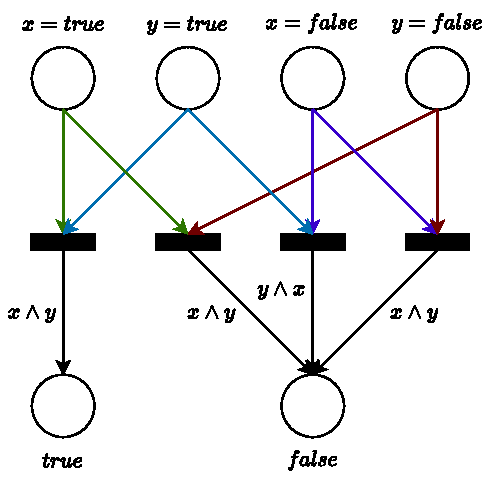
\includegraphics[width=.7\textwidth]{img/logical-and-1.pdf}
    \caption{Petri Net model of logical and.}
    \label{fig: exercises - logical and}
\end{figure}

\highspace
\textbf{\underline{Solution 2}.} The model of the negation $x$ depends on the negation logic table:

\begin{table}[!htp]
    \centering
    \begin{tabular}{@{} c c @{}}
        \toprule
        $x$ & $\lnot x$ \\
        \midrule
        \texttt{True} & \texttt{False} \\
        \texttt{False} & \texttt{True} \\
        \bottomrule
    \end{tabular}
\end{table}

\noindent
The Petri Net model is exposed in the Figure~\ref{fig: exercises - logical not}.

\begin{figure}[!htp]
    \centering
    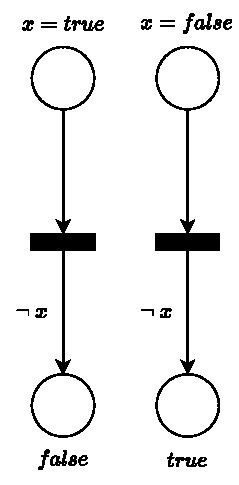
\includegraphics[width=.35\textwidth]{img/logical-and-2.pdf}
    \caption{Petri Net model of logical not.}
    \label{fig: exercises - logical not}
\end{figure}

\highspace
\textbf{\underline{Solution 3}.} To combine the previous two models, we can extend the first model (Figure~\ref{fig: exercises - logical and}) with the second (Figure~\ref{fig: exercises - logical not}) in a very simple way. See the final Petri Net model in the Figure~\ref{fig: exercises - logical and, not}.

\begin{figure}[!htp]
    \centering
    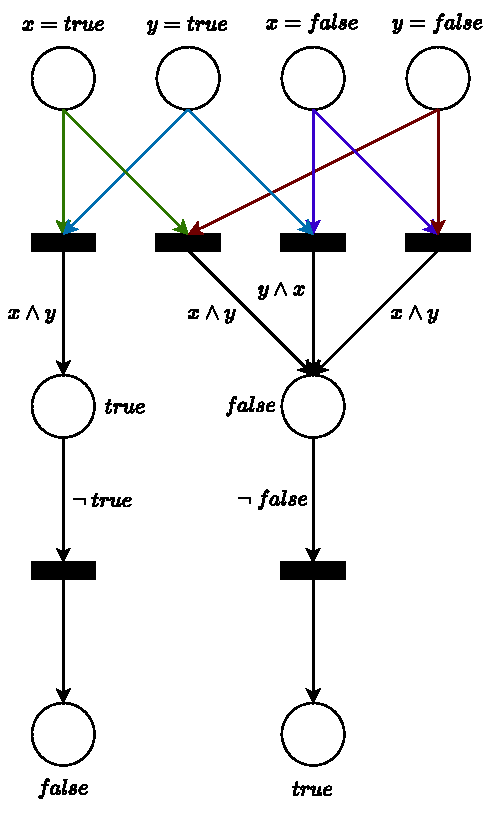
\includegraphics[width=.7\textwidth]{img/logical-and-3.pdf}
    \caption{Petri Net model of logical $\land$ and $\lnot$.}
    \label{fig: exercises - logical and, not}
\end{figure}